\chapter{Random walk su grafi: hitting, commute e cover time}

Il \emph{random walk} su un grafo è l'esempio più naturale di catena di Markov: gli stati
sono i vertici e a ogni passo si sceglie a caso uno degli archi incidenti al vertice
corrente. In questo capitolo vediamo che cosa il teorema fondamentale delle catene di
Markov dice di questa catena --- la distribuzione stazionaria è proporzionale al grado ---
e introduciamo le tre grandezze con cui se ne misura il costo: \emph{hitting time},
\emph{commute time} e \emph{cover time}.

\section{La catena di Markov associata a un grafo}

\scan{83}

\begin{osservazione}[Richiamo: il teorema fondamentale delle catene di Markov]
  Ogni catena di Markov irriducibile, finita e aperiodica gode delle seguenti proprietà:
  tutti i suoi stati sono ergodici (e lo è dunque la catena stessa); esiste un'unica
  distribuzione stazionaria $\vec{\pi}$, e per essa $\pi_i > 0$ per ogni
  $i \in \{1,\dots,n\}$; per ogni stato $i$ valgono $f_{i,i} = 1$ e $h_{i,i} = 1/\pi_i$;
  infine, detto $N(i,t)$ il numero medio di volte in cui la catena visita lo stato $i$ nei
  primi $t$ passi, $\lim_{t\to\infty} N(i,t)/t = \pi_i$.

  Il Teorema~\ref{thm:mc-fondamentale} è stato enunciato e discusso nel capitolo precedente;
  qui ne useremo due conseguenze: l'\emph{unicità} della distribuzione stazionaria e l'identità
  $h_{i,i} = 1/\pi_i$ fra tempo medio di ritorno in uno stato e probabilità stazionaria
  dello stato.
\end{osservazione}

Sia dunque $G = (V,E)$ un grafo \emph{connesso}, \emph{non orientato} e \emph{non
bipartito}, con
\[
  \abs{V} = n , \qquad \abs{E} = m .
\]
Queste tre ipotesi restano in vigore per tutto il capitolo. Per $u \in V$ indichiamo con
$\Gamma(u)$ l'insieme dei vicini di $u$ e con $d(u) = \abs{\Gamma(u)}$ il suo grado.
L'ultima ipotesi --- la non bipartitezza --- serve a garantire la \emph{non periodicità}
(cioè l'aperiodicità) della catena che stiamo per costruire, ed è l'oggetto
dell'osservazione che chiude la sezione; la connessione serve all'irriducibilità e la
finitezza è ovvia.

\begin{definizione}[Random walk su un grafo]\label{def:random-walk-grafo}
  La catena di Markov $M_G$ associata a $G$ è definita così:
  \begin{itemize}
    \item gli \textbf{stati} sono i \textbf{vertici} del grafo;
    \item per ogni $u, v \in V$ la probabilità di transizione è
      \[
        P_{u,v} \;=\;
        \begin{cases}
          \dfrac{1}{d(u)} & \text{se } (u,v) \in E,\\[8pt]
          0 & \text{altrimenti.}
        \end{cases}
      \]
  \end{itemize}
  Il passo elementare è dunque: dal vertice corrente $u$ si sceglie uniformemente a caso
  uno dei $d(u)$ archi incidenti e lo si attraversa.
\end{definizione}

\begin{figure}[H]
  \centering
  % p83-transizioni-mg -- pag. 83
% Un passo del random walk M_G a partire dal vertice u: dei d(u) archi incidenti
% se ne sceglie uno uniformemente a caso, dunque P_{u,v} = 1/d(u).
% Il quaderno disegna tre archi a ventaglio; qui i tre archi restano, ma fra l'uno
% e l'altro si aggiungono i puntini che segnalano i vicini omessi, cosi' che l'arco
% di cerchio possa davvero contare d(u) archi.  Grafo non orientato: niente frecce.
\begin{tikzpicture}[
    x=1cm, y=1cm, line join=round, line cap=round,
    font=\footnotesize,
    nodo/.style   = {circle, draw, line width=0.7pt, fill=white,
                     inner sep=0pt, minimum size=5pt},
    nodov/.style  = {circle, draw, line width=0.8pt, fill=white,
                     inner sep=0pt, minimum size=7pt},
    arco/.style   = {line width=0.7pt},
    conta/.style  = {gray!70!black, line width=0.6pt},
  ]

  % ---- il vertice corrente ------------------------------------------------
  \node[nodov] (u) at (0,0) {};
  \node[anchor=north east, inner sep=2pt] at (u.south west) {$u$};

  % ---- il ventaglio dei vicini (tre archi, campione dei d(u)) -------------
  \def\Ra{2.55}
  \node[nodo]  (w1) at (48:\Ra) {};
  \node[nodov] (v)  at (-2:\Ra) {};
  \node[nodo]  (w2) at (-52:\Ra) {};

  \node[anchor=west, inner sep=3pt] at (v.east) {$v$};

  \draw[arco] (u) -- (w1);
  \draw[arco] (u) -- (v);
  \draw[arco] (u) -- (w2);

  % ---- i vicini omessi: puntini fra un arco e l'altro ---------------------
  \foreach \ang in {32,23,14}{\fill[gray!70!black] (\ang:2.45) circle (0.65pt);}
  \foreach \ang in {-18,-27,-36}{\fill[gray!70!black] (\ang:2.45) circle (0.65pt);}

  % ---- la probabilita' di scegliere l'arco u--v ---------------------------
  \node[anchor=south, inner sep=2.5pt] at (-2:1.5) {$\dfrac{1}{d(u)}$};

  % ---- arco di cerchio che "conta" gli archi incidenti a u ----------------
  \draw[conta] (58:1.05) arc[start angle=58, end angle=-62, radius=1.05];
  \node[anchor=north east, inner sep=1pt] at (-64:1.05) {$d(u)$};

\end{tikzpicture}

  \caption{Un passo di $M_G$ a partire da $u$: dei $d(u)$ archi incidenti se ne sceglie
  uno uniformemente a caso, dunque $P_{u,v} = 1/d(u)$ per ogni vicino $v$ di $u$.}
  \label{fig:transizioni-mg}
\end{figure}

\begin{osservazione}[$M_G$ è aperiodica]
  La \emph{periodicità} di un vertice (cioè di uno stato) $v$ è
  \[
    T_v \;=\; \gcd\bigl\{\, \text{lunghezze di tutti i cammini chiusi (cicli) da } v \,\bigr\}.
  \]
  Nel caso di $M_G$:
  \begin{itemize}
    \item ogni arco di $G$, essendo non orientato, dà luogo alle due transizioni opposte
      $u \to v$ e $v \to u$: abbiamo dunque cicli di lunghezza $2$;
    \item $G$ non è bipartito, quindi ci sono anche cicli di lunghezza dispari, diciamo
      $2k+1$.
  \end{itemize}
  Ne segue
  \[
    T_v \;=\; \gcd(2,\, 2k+1) \;=\; 1
  \]
  per ogni $v$, cioè $M_G$ è aperiodica.

  Perché l'argomento sia completo occorre però che entrambi i cammini chiusi passino per lo
  \emph{stesso} vertice $v$. Per il primo non c'è nulla da dire: $G$ è connesso, quindi ogni
  vertice ha almeno un arco incidente. Per il secondo: se il ciclo dispari non passa per
  $v$, si raggiunge un suo vertice $w$ con un cammino di lunghezza $\ell$, si percorre il
  ciclo e si torna indietro lungo lo stesso cammino, ottenendo un cammino chiuso da $v$ di
  lunghezza $2\ell + (2k+1)$, ancora dispari. La connessione di $G$ garantisce dunque che
  ogni vertice stia su cammini chiusi di lunghezza $2$ e di lunghezza dispari.
\end{osservazione}

\begin{figure}[H]
  \centering
  % p83-arco-ciclo2 -- pag. 83
% Ogni arco non orientato di G diventa, in M_G, la coppia di transizioni opposte
% u -> v e v -> u: un cammino chiuso di lunghezza 2.  Due pannelli separati da =>.
% Nel quaderno i due punti non sono etichettati: qui si aggiungono u, v e i nomi
% delle due probabilita' di transizione.
\begin{tikzpicture}[
    x=1cm, y=1cm, line join=round, line cap=round,
    font=\footnotesize,
    punto/.style = {circle, fill, inner sep=0pt, minimum size=3pt},
    arco/.style  = {line width=0.7pt},
    tran/.style  = {line width=0.7pt, -{Latex[length=1.9mm,width=1.5mm]}},
    didasc/.style= {gray!70!black, anchor=north, inner sep=1pt},
  ]

  % ================= pannello di sinistra: l'arco di G =====================
  \node[punto] (a) at (0,0)   {};
  \node[punto] (b) at (1.7,0) {};
  \node[anchor=east, inner sep=3pt] at (a.west) {$u$};
  \node[anchor=west, inner sep=3pt] at (b.east) {$v$};

  \draw[arco] (a) to[bend left=45] (b);

  \node[didasc] at (0.85,-0.95) {in $G$: un arco};

  % ================= freccia di implicazione ==============================
  \node at (2.95,0.14) {$\Longrightarrow$};

  % ================= pannello di destra: il 2-ciclo di M_G ================
  \node[punto] (c) at (4.2,0) {};
  \node[punto] (d) at (5.9,0) {};
  \node[anchor=east, inner sep=3pt] at (c.west) {$u$};
  \node[anchor=west, inner sep=3pt] at (d.east) {$v$};

  \draw[tran] (c) to[bend left=45] node[above,inner sep=1.5pt] {$P_{u,v}$} (d);
  \draw[tran] (d) to[bend left=45] node[below,inner sep=1.5pt] {$P_{v,u}$} (c);

  \node[didasc] at (5.05,-0.95) {in $M_G$: un ciclo di lunghezza $2$};

\end{tikzpicture}

  \caption{Ogni arco non orientato di $G$ diventa, in $M_G$, una coppia di transizioni
  opposte, cioè un cammino chiuso di lunghezza $2$.}
  \label{fig:arco-ciclo2}
\end{figure}

\scan{84}

Le tre ipotesi del teorema fondamentale sono dunque tutte soddisfatte da $M_G$:
\[
  \left.
  \begin{array}{l}
    M_G \text{ è aperiodica} \\[2pt]
    M_G \text{ è finita} \\[2pt]
    M_G \text{ è irriducibile}
  \end{array}
  \right\}
  \;\Longrightarrow\;
  \text{posso applicare il teorema.}
\]
L'aperiodicità è quella appena verificata, la finitezza viene dal fatto che gli stati sono
gli $n$ vertici del grafo e l'irriducibilità dalla connessione di $G$.

\section{Intermezzo: mescolare un mazzo di carte}

\begin{esercizio}[Mescolare un mazzo di carte]\label{ex:mazzo-carte}
  Come si mescola un mazzo di carte? Ovvero: quanto vale il \emph{mixing time} della catena
  di Markov che descrive il mescolamento?
\end{esercizio}

Gli stati della catena sono le permutazioni del mazzo: per un mazzo di $K = 52$ carte sono
\[
  K! \;=\; 52! \;\approx\; 10^{68}
\]
possibili stati.

Il mescolamento che consideriamo è il \emph{top-in-at-random}: a ogni passo si toglie la
carta in cima al mazzo e la si reinserisce in una delle $K$ posizioni possibili, scelta
uniformemente a caso.

\begin{figure}[H]
  \centering
  % top-in-at-random -- pag. 84
% Il mescolamento top-in-at-random: il mazzo e' visto di taglio (una carta = un
% segmento orizzontale).  Pannello superiore: la carta in cima viene tolta e
% reinserita in una posizione scelta a caso; B e' la carta in fondo al mazzo.
% Pannello inferiore: dopo un certo numero di passi B e' risalita e le carte che
% le sono passate sotto sono in ordine uniformemente casuale (l'invariante).
% Nel quaderno i due mazzi hanno 6 e 7 carte: qui entrambi ne hanno 7, perche' il
% numero di carte non cambia lungo il mescolamento.
\begin{tikzpicture}[
    x=1cm, y=1cm, line join=round, line cap=round,
    font=\footnotesize,
    carta/.style  = {line width=0.8pt},
    cartaB/.style = {line width=1.7pt},
    frec/.style   = {line width=0.7pt, -{Latex[length=2mm,width=1.6mm]}},
    graffa/.style = {decorate, decoration={brace, amplitude=4pt},
                     gray!70!black, line width=0.6pt},
  ]

  \def\W{1.9}     % larghezza del mazzo
  \def\P{0.3}     % passo verticale fra due carte

  % =================== intestazione =======================================
  \node[anchor=south] at (1.55, 0.45) {\emph{top-in-at-random}};

  % =================== pannello superiore: il mazzo iniziale ==============
  % sette carte, y = 0, -0.3, ..., -1.8;  B e' l'ultima
  \foreach \i in {0,...,5}{\draw[carta] (0,-\i*\P) -- (\W,-\i*\P);}
  \draw[cartaB] (0,-6*\P) -- (\W,-6*\P);
  \node[anchor=east, inner sep=4pt] at (0,-6*\P) {$B$};

  % la carta in cima esce e rientra in una posizione a caso
  \draw[frec] (\W,0.03) .. controls (2.85,0.14) and (2.95,-1.02) .. (1.62,-1.06);
  \node[anchor=west, inner sep=2pt] at (2.62,-0.42) {a caso};

  % =================== transizione fra i due pannelli =====================
  \draw[line width=1.5pt, -{Latex[length=3mm,width=2.6mm]}]
        (\W/2,-2.24) -- (\W/2,-2.86);
  \node[anchor=west, inner sep=5pt, align=left, gray!70!black]
        at (\W/2,-2.55) {dopo un certo\\numero di passi};

  % =================== pannello inferiore: dopo alcuni passi ==============
  % sette carte, y = -3.3, ..., -5.1;  B e' la quarta (tre sopra, tre sotto)
  \def\Y{-3.3}
  \foreach \i in {0,1,2}{\draw[carta] (0,\Y-\i*\P) -- (\W,\Y-\i*\P);}
  \draw[cartaB] (0,\Y-3*\P) -- (\W+0.22,\Y-3*\P);
  \node[anchor=east, inner sep=4pt] at (0,\Y-3*\P) {$B$};
  \foreach \i in {4,5,6}{\draw[carta] (0,\Y-\i*\P) -- (\W,\Y-\i*\P);}

  % le carte finite sotto B sono in ordine uniformemente casuale
  \draw[graffa] (\W+0.42,\Y-3.6*\P) -- (\W+0.42,\Y-6.4*\P);
  \node[anchor=west, inner sep=8pt] at (\W+0.42,\Y-5*\P) {a caso};

\end{tikzpicture}

  \caption{Il mescolamento \emph{top-in-at-random}: la carta in cima al mazzo viene
  reinserita in una posizione scelta uniformemente a caso. In alto la situazione iniziale,
  con la carta $B$ in fondo al mazzo; in basso, dopo un certo numero di passi, $B$ è
  risalita e le carte che le sono passate sotto si trovano in ordine uniformemente
  casuale.}
  \label{fig:top-in-at-random}
\end{figure}

Sia $B$ la carta che all'inizio si trova in fondo al mazzo. Vogliamo valutare il numero $T$
di operazioni che servono per portare $B$ in prima posizione.

Supponiamo che sotto $B$ ci siano già $i-1$ carte. La carta reinserita finisce sotto $B$
esattamente quando la posizione estratta è una delle $i$ che stanno al di sotto di $B$, il
che accade con probabilità
\[
  p_i \;=\; \frac{i}{K}
  \qquad\text{cioè, via via,}\quad \frac{1}{K},\ \frac{2}{K},\ \dots,\ \frac{K-1}{K}.
\]
Detto $T_i$ il numero di passi necessari per passare da $i-1$ a $i$ carte sotto $B$, la
variabile $T_i$ è geometrica di parametro $p_i$, e quindi, per il conto già fatto sul valore
atteso di una variabile geometrica,
\[
  \E[T_i] \;=\; \frac{1}{p_i} \;=\; \frac{K}{i}.
\]

La carta $B$ arriva in prima posizione quando tutte le altre $K-1$ carte le sono passate
sotto, dunque
\[
  T \;=\; T_1 + T_2 + \dots + T_{K-1}
\]
e, per linearità del valore atteso,
\[
  \E[T] \;=\; \sum_{i=1}^{K-1} \E[T_i]
        \;=\; K \sum_{i=1}^{K-1} \frac{1}{i}
        \;=\; K\,H_{K-1}
        \;=\; \Oh(K \log K),
\]
dove $H_K = \sum_{i=1}^{K} 1/i$ è il $K$-esimo numero armonico: è di nuovo il conto del
\emph{coupon collector}.

\begin{osservazione}
  Un solo passo in più basta a concludere il mescolamento: nell'istante in cui $B$, arrivata
  in cima, viene a sua volta reinserita in una posizione casuale, tutte le $K$ carte sono
  state collocate a caso e il mazzo è uniformemente mescolato. Contando anche quel passo si
  ottiene
  \[
    \sum_{i=1}^{K} \frac{K}{i} \;=\; K\,H_K \;\approx\; K \ln K
  \]
  (l'addendo con $i=K$ vale esattamente $1$ ed è proprio il passo finale). Per $K = 52$
  servono dunque in media $52\,H_{52} \approx 236$ mescolate: l'ordine di grandezza è
  $K \ln K \approx 205$, e i circa $30$ passi di differenza sono il termine $\gamma K$ che
  l'approssimazione $H_K \approx \ln K$ trascura ($\gamma \approx 0{,}577$ è la costante di
  Eulero--Mascheroni).
\end{osservazione}

\section{La distribuzione stazionaria del random walk}

\begin{lemma}[Distribuzione stazionaria di un random walk]\label{lem:stazionaria-grado}
  Sia $M_G$ la catena associata al grafo $G = (V,E)$, con $\abs{V} = n$ e $\abs{E} = m$.
  Allora
  \[
    \forall v \in V \qquad \pi_v \;=\; \frac{d(v)}{2m}.
  \]
\end{lemma}

\begin{dimostrazione}
  Dobbiamo trovare $\vec{\pi}$ soluzione di
  \[
    \vec{\pi} \;=\; \vec{\pi}\,P ,
  \]
  e per farlo basta verificare che il vettore di componenti $d(v)/2m$, al variare di
  $v \in V$, soddisfa questa equazione, cioè che per ogni $u \in V$ vale
  $\pi_u = \sum_{v \in V} \pi_v P_{v,u}$.

  \scan{85}
  Poiché $P_{v,u} \neq 0$ soltanto se $v \in \Gamma(u)$, e in tal caso
  $P_{v,u} = 1/d(v)$,
  \[
    \frac{d(u)}{2m}
    \;\overset{?}{=}\;
    \sum_{v \in \Gamma(u)} \frac{d(v)}{2m} \cdot P_{v,u}
    \;=\;
    \sum_{v \in \Gamma(u)} \frac{d(v)}{2m} \cdot \frac{1}{d(v)}
    \;=\;
    \frac{1}{2m} \sum_{v \in \Gamma(u)} 1
    \;=\;
    \frac{d(u)}{2m} \,,
  \]
  perché la somma ha esattamente $\abs{\Gamma(u)} = d(u)$ addendi, uno per ogni vicino di $u$.

  Il vettore così definito è inoltre una distribuzione di probabilità: ogni arco contribuisce
  al grado di entrambi i suoi estremi, quindi $\sum_{v \in V} d(v) = 2m$ e di conseguenza
  $\sum_{v \in V} \pi_v = 1$.
\end{dimostrazione}

Ergo, per ogni $v \in V$, il tempo medio di ritorno in $v$ --- che per il teorema
fondamentale è il reciproco della probabilità stazionaria --- vale
\[
  h_{v,v} \;=\; \frac{1}{\pi_v} \;=\; \frac{2m}{d(v)} \,.
\]

\section{Hitting time, commute time e cover time}

\begin{definizione}[Hitting time, commute time, cover time]\label{def:tempi}
  Si consideri il random walk su $G = (V,E)$.
  \begin{itemize}
    \item $h_{u,v}$ --- \emph{hitting time}: numero medio di passi per andare da $u$ a $v$.
    \item $C_{u,v}$ --- \emph{commute time}:
      \[
        h_{u,v} + h_{v,u} \;=\; C_{u,v} \;=\; C_{v,u} \,.
      \]
    \item $C_u(G)$ --- tempo medio per tornare a $u$ dopo aver visitato l'intero $G$
      partendo da $u$.
    \item $C(G)$ --- \emph{cover time} di $G$:
      \[
        C(G) \;=\; \max_{u} \, C_u(G) \,.
      \]
  \end{itemize}
\end{definizione}

\begin{domanda}\label{q:simmetria-hitting}
  Vale $h_{u,v} = h_{v,u}$?
\end{domanda}

Si consideri il \emph{lollipop graph} $L_n$: una clique $K_{n/2}$ alla quale è incollato,
nel vertice $u$, un cammino di $n/2$ vertici che termina in $v$.

\begin{figure}[H]
  \centering
  % p85-lollipop -- pag. 85 (la stessa figura torna a p. 88, deduplicata)
% Il lollipop graph L_n: la clique K_{n/2} e' rappresentata astrattamente da un
% cerchio (vertici e archi interni non si disegnano); nel vertice u -- l'unico
% pieno, sul bordo destro del cerchio -- e' incollato un cammino di n/2 vertici
% che termina in v.  In tutto n vertici.
% Il quaderno e' tutto a penna blu: qui si usa il nero come nelle altre figure.
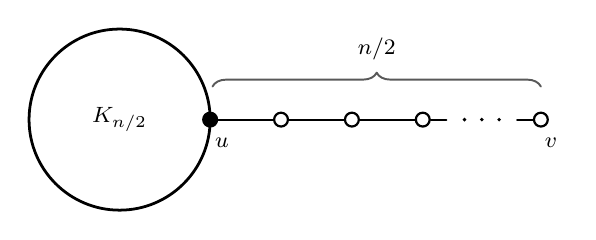
\begin{tikzpicture}[
    x=1cm, y=1cm, line join=round, line cap=round,
    font=\footnotesize,
    nodo/.style   = {circle, draw, line width=0.8pt, fill=white,
                     inner sep=0pt, minimum size=5pt},
    nodou/.style  = {circle, draw, fill=black, line width=0.8pt,
                     inner sep=0pt, minimum size=5pt},
    arco/.style   = {line width=0.8pt},
    graffa/.style = {decorate, decoration={brace, amplitude=5pt},
                     gray!70!black, line width=0.7pt},
  ]

  % =================== la clique K_{n/2} ==================================
  \draw[arco, line width=1pt] (0,0) circle (1.15);
  \node at (0,0) {$K_{n/2}$};

  % =================== il bastoncino: cammino di n/2 vertici ==============
  \node[nodou] (u)  at (1.15,0) {};
  \node[nodo]  (p1) at (2.05,0) {};
  \node[nodo]  (p2) at (2.95,0) {};
  \node[nodo]  (p3) at (3.85,0) {};
  \node[nodo]  (v)  at (5.35,0) {};

  \draw[arco] (u)  -- (p1);
  \draw[arco] (p1) -- (p2);
  \draw[arco] (p2) -- (p3);

  % i vertici omessi
  \draw[arco] (p3) -- (4.15,0);
  \foreach \x in {4.38,4.60,4.82}{\fill (\x,0) circle (0.7pt);}
  \draw[arco] (5.05,0) -- (v);

  \node[anchor=north, inner sep=4pt] at (1.30,-0.09) {$u$};
  \node[anchor=north, inner sep=4pt] at (5.48,-0.09) {$v$};

  % =================== la graffa che misura il bastoncino =================
  \draw[graffa] (1.18,0.42) -- (5.35,0.42)
        node[midway, above=6pt, black] {$n/2$};

\end{tikzpicture}

  \caption{Il \emph{lollipop graph} $L_n$: una clique $K_{n/2}$ alla quale è incollato,
  nel vertice $u$, un cammino di $n/2$ vertici che termina in $v$; in tutto $n$ vertici.}
  \label{fig:lollipop}
\end{figure}

\scan{86}

Dimostreremo che su $L_n$ l'hitting time non è affatto simmetrico:
\[
  h_{u,v} \;=\; \Th(n^{3}),
  \qquad\text{mentre}\qquad
  h_{v,u} \;=\; \Th(n^{2}).
\]
I due versi differiscono dunque di un fattore $n$: la risposta alla
Domanda~\ref{q:simmetria-hitting} è negativa.

Dimostreremo anche che sul grafo completo $K_n$ il cover time vale
\[
  C_u(K_n) \;=\; \Th(n \log n) \qquad\text{per ogni } u \in V .
\]

\begin{osservazione}
  Su $K_n$ ogni vertice ha $n-1$ vicini, tutti equiprobabili, dunque il numero di passi
  necessari per raggiungere un fissato $v \neq u$ è una variabile geometrica di parametro
  $1/(n-1)$ e
  \[
    h_{u,v} \;=\; n-1 \;=\; \Th(n) \qquad \text{per ogni } u \neq v :
  \]
  sul grafo completo l'hitting time è lineare e uguale per tutte le coppie. È invece il
  numero di passi necessari a \emph{visitare tutti} i vertici a valere
  $(n-1)H_{n-1} = \Th(n \log n)$: è il conto del collezionista di figurine.
\end{osservazione}

\paragraph{Morale.} Non è ovvio come ragionare per stimare $C_u(G)$ e $C(G)$. Lo strumento
classico è l'analogia fra passeggiate aleatorie su grafi e reti di resistenze, esposta in
«\emph{Random Walks and Electric Networks}» di P.~G.~Doyle e J.~L.~Snell (1984); qui
seguiamo invece una strada elementare, che parte dal commute time di un singolo arco.

\section{Il commute time lungo un arco}

\begin{lemma}[Commute time lungo un arco]\label{lem:commute-arco}
  Sia $G = (V,E)$ come sopra, con $\abs{E} = m$. Se $u$ e $v$ sono \emph{adiacenti}, cioè
  $(u,v) \in E$, allora
  \[
    C_{u,v} \;=\; h_{u,v} + h_{v,u} \;\le\; 2m .
  \]
\end{lemma}

L'ipotesi di adiacenza è essenziale: se cade, la disuguaglianza può essere falsa. Sul
lollipop graph, per esempio, $h_{u,v} + h_{v,u} = \Th(n^{3})$ mentre $2m = \Th(n^{2})$,
perché la clique $K_{n/2}$ ha già $\Th(n^{2})$ archi.

\begin{dimostrazione}
  Introduciamo una catena di Markov ausiliaria i cui stati sono gli \emph{archi orientati}
  di $G$: ogni arco non orientato di $G$ dà luogo ai due stati $(u,v)$ e $(v,u)$, per un
  totale di $2m$ stati. In questa dimostrazione, dunque, la scrittura $(u,v)$ denota un arco
  \emph{orientato}; lo stato $(u,v)$ va letto come «la passeggiata ha appena attraversato
  l'arco da $u$ a $v$», e si trova quindi nel vertice $v$.

  La matrice di transizione $Q$ della catena così introdotta è
  \[
    Q_{(u,v),(v,w)} \;=\; P_{v,w} \;=\; \frac{1}{d(v)}
    \qquad (w \in \Gamma(v)),
  \]
  e tutte le altre entrate sono nulle, perché dallo stato $(u,v)$ si può passare soltanto a
  uno stato della forma $(v,w)$, e lo si fa con la stessa probabilità con cui il random walk
  su $G$, trovandosi in $v$, sceglie il vicino $w$.

  \medskip
  \textbf{Osservazione: $Q$ è \emph{doubly stochastic}}, cioè righe e colonne sommano a $1$.
  \begin{itemize}
    \item \emph{Righe.} Fissato lo stato $(u,v)$,
      \[
        \sum_{w \in \Gamma(v)} Q_{(u,v),(v,w)}
        \;=\; \sum_{w \in \Gamma(v)} \frac{1}{d(v)}
        \;=\; \frac{d(v)}{d(v)} \;=\; 1 .
      \]
    \item \emph{Colonne.} Fissato lo stato $(v,w)$, nella somma su tutti gli stati $(x,y)$
      sopravvivono soltanto i termini con $y = v$ e $x \in \Gamma(v)$, e quindi
      \[
        \sum_{x \in V} \; \sum_{y \in \Gamma(x)} Q_{(x,y),(v,w)}
        \;=\; \sum_{x \in \Gamma(v)} Q_{(x,v),(v,w)}
        \;=\; \sum_{x \in \Gamma(v)} \frac{1}{d(v)}
        \;=\; \frac{d(v)}{d(v)} \;=\; 1 .
      \]
  \end{itemize}

  \medskip
  \scan{87}
  Anche questa catena soddisfa le ipotesi del teorema fondamentale: è \emph{finita}, perché
  ha $2m$ stati; è \emph{irriducibile}, perché nello stato $(u,v)$ la passeggiata si trova in
  $v$ e, essendo $G$ connesso, può raggiungere qualunque vertice $x$ e attraversare poi un
  qualunque arco $x \to y$, arrivando nello stato $(x,y)$; ed è \emph{aperiodica}, perché
  $(u,v) \to (v,u) \to (u,v)$ è un cammino chiuso di lunghezza $2$, mentre un cammino chiuso
  di lunghezza dispari da $v$ a $v$ --- che esiste, per quanto visto sopra, perché $G$ non è
  bipartito --- seguito da $v \to u \to v$ riporta in $(u,v)$ dopo un numero dispari di passi.

  La distribuzione stazionaria di una matrice \emph{doubly stochastic} è quella uniforme.
  Basta dunque verificare che $\vec{\pi} = \vec{\pi}\,Q$ per $\vec{\pi}$ uniforme e poi
  invocare il teorema fondamentale delle catene di Markov, che garantisce l'unicità della
  distribuzione stazionaria.

  Poiché le colonne di $Q$ sommano a $1$, «mi piacerebbe» che fosse $\pi_x = 1$ per ogni
  stato $x$: il vettore di tutti $1$ è in effetti fissato da $Q$. Ma così
  $\sum_x \pi_x \neq 1$, e $\vec{\pi}$ non sarebbe una distribuzione di probabilità. Il rimedio
  è normalizzare: poniamo
  \[
    \pi_x \;=\; \frac{1}{\text{numero degli stati}} \;=\; \frac{1}{2m},
  \]
  visto che gli stati della catena sono i $2m$ archi orientati di $G$.

  Le due verifiche sono ora immediate. La normalizzazione:
  \[
    \sum_x \pi_x \;=\; \sum_x \frac{1}{2m} \;=\; \frac{2m}{2m} \;=\; 1 ;
  \]
  la stazionarietà: per ogni stato $x$,
  \[
    \sum_y \pi_y\, Q_{y,x}
    \;=\; \frac{1}{2m} \underbrace{\Bigl(\sum_y Q_{y,x}\Bigr)}_{=\;1\ (Q \text{ doubly stochastic})}
    \;=\; \frac{1}{2m}
    \;=\; \pi_x .
  \]

  Per l'unicità della distribuzione stazionaria si conclude allora che, per ogni arco
  orientato $(u,v)$, si ha $\pi_{(u,v)} = 1/(2m)$ e quindi, per l'identità fra tempo medio di
  ritorno e probabilità stazionaria,
  \[
    h_{(u,v),(u,v)} \;=\; \frac{1}{\pi_{(u,v)}} \;=\; 2m .
  \]

  Resta da collegare questo tempo di ritorno ai due hitting time $h_{u,v}$ e $h_{v,u}$ sui
  \emph{vertici}. La quantità $h_{(u,v),(u,v)}$ è il tempo medio che intercorre fra una visita
  dello stato $(u,v)$ e la visita successiva dello stesso stato: appena attraversato l'arco
  $u \to v$ la passeggiata si trova in $v$, vaga per il grafo, prima o poi ritorna in $u$ e
  solo allora può attraversare una seconda volta l'arco $u \to v$ (Figura~\ref{fig:ritorno-arco}).

  Spezzando il tragitto nel primo arrivo in $u$ e in ciò che segue si ottiene
  \[
    2m \;=\; h_{(u,v),(u,v)} \;\ge\; h_{v,u} + h_{u,v} :
  \]
  tornare in $u$ partendo da $v$ costa in media $h_{v,u}$ e, una volta in $u$, per rivedere
  lo stato $(u,v)$ la passeggiata deve come minimo ritrovarsi in $v$, il che costa in media
  almeno $h_{u,v}$. Dunque
  \[
    h_{u,v} + h_{v,u} \;\le\; 2m
    \qquad\text{per } (u,v) \in E ,
  \]
  che è la tesi.
\end{dimostrazione}

\begin{figure}[H]
  \centering
  % p87-ritorno-arco -- pag. 87
% Primo ritorno nello stato (u,v) della catena sugli archi orientati:
%   u -> v  (prima traversata)  ~>  vagabondaggio nel grafo fino a rientrare in u
%   ~>  u -> v  (seconda traversata).
% Visualizza la decomposizione  h_{(u,v),(u,v)} >= h_{v,u} + h_{u,v}.
% Il grafo resta implicito: la curva chiusa e' la traiettoria della passeggiata,
% non un arco di G.
\begin{tikzpicture}[
    x=1cm, y=1cm,
    vert/.style     = {circle, fill=graydark, inner sep=0pt, minimum size=4pt},
    traversa/.style = {draw=accent, line width=1.1pt, line cap=round,
                       -{Stealth[length=5pt,width=4pt]}},
    vaga/.style     = {draw=graydark, line width=0.6pt, line cap=round,
                       line join=round},
    et/.style       = {font=\footnotesize},
  ]

  \coordinate (u) at (0.00, 0.00);
  \coordinate (v) at (2.40, 1.05);

  % ---- il vagabondaggio: un'unica traiettoria che esce da v, gira a lungo
  %      per il grafo e rientra in u ------------------------------------------
  \draw[vaga, -{Stealth[length=5pt,width=4pt]}]
       (2.50, 1.09)
       .. controls ( 4.70, 1.30) and ( 5.60,-0.30) .. ( 4.90,-1.60)
       .. controls ( 4.20,-2.90) and ( 2.20,-3.40) .. ( 0.40,-3.00)
       .. controls (-1.30,-2.60) and (-2.10,-1.30) .. (-1.50,-0.55)
       .. controls (-1.05,-0.40) and ( 0.90,-0.60) .. ( 1.90,-0.85)
       .. controls ( 3.10,-1.55) and ( 3.00,-2.45) .. ( 1.70,-2.55)
       .. controls ( 0.55,-2.65) and (-0.62,-2.05) .. (-0.78,-1.35)
       .. controls (-0.88,-0.80) and (-0.50,-0.35) .. (-0.10,-0.10);

  % ---- le due traversate dell'arco u -> v ------------------------------------
  \draw[traversa] (u) to[bend left=16]  (v);
  \draw[traversa] (u) to[bend right=16] (v);

  \node[vert] at (u) {};
  \node[vert] at (v) {};

  \node[et, anchor=east,  xshift=-4pt] at (u) {$u$};
  \node[et, anchor=south, yshift=4pt]  at (v) {$v$};

  \node[et, rotate=23.6, anchor=south] at (1.13, 0.76) {1\textsuperscript{a} traversata};
  \node[et, rotate=23.6, anchor=north] at (1.30, 0.29) {2\textsuperscript{a} traversata};

  \node[et, anchor=north, align=center] at (1.70,-3.30)
       {vagabondaggio nel grafo\\ prima del rientro in $u$ \ ($h_{v,u}$)};

\end{tikzpicture}

  \caption{Il ritorno nello stato $(u,v)$ della catena sugli archi orientati: dopo la prima
  traversata di $u \to v$ la passeggiata vaga per il grafo, rientra in $u$ e attraversa una
  seconda volta $u \to v$.}
  \label{fig:ritorno-arco}
\end{figure}

\section{Una stima del cover time}

\scan{88}

Il lemma appena dimostrato --- $C_{u,v} = h_{u,v} + h_{v,u} \le 2m$ per ogni arco
$(u,v) \in E$ --- si propaga da un singolo arco a tutto il grafo e fornisce la stima del
cover time.

\begin{teorema}[Stima del cover time]\label{thm:cover-time}
  Sia $G = (V,E)$ come sopra, con $n = \abs{V}$ e $m = \abs{E}$. Allora
  \[
    C(G) \;\le\; 2m\,(n-1) \,.
  \]
\end{teorema}

\begin{dimostrazione}
  Si fissi uno spanning tree $T$ di $G$ e lo si percorra con un tour euleriano dell'albero
  raddoppiato: partendo da un vertice qualsiasi $u$ si toccano tutti i vertici e si torna in
  $u$ attraversando ciascuno degli $n-1$ archi di $T$ una volta per verso. Il costo atteso di
  questo tour è la somma dei commute time dei suoi archi, e ogni arco di $T$ è un arco di
  $G$, al quale si applica il Lemma~\ref{lem:commute-arco}: per ogni $u \in V$
  \[
    C_u(G) \;\le\; \sum_{(x,y) \in T} C_{x,y} \;\le\; (n-1) \cdot 2m \,,
  \]
  e passando al massimo su $u$ si ottiene la tesi.
\end{dimostrazione}

\begin{esempio}[I due casi estremi]
  \textbf{Cammino.} Se $G$ è un cammino su $n$ vertici (Figura~\ref{fig:cammino}), allora
  $m = n-1$ e la stima dà
  \[
    2(n-1)(n-1) \;\in\; \Th(n^2) \,.
  \]
  Il cammino è bipartito, e cade quindi fuori dalle ipotesi permanenti fissate all'inizio del
  capitolo; la stima vale lo stesso, perché di quelle ipotesi la catena di deduzioni usa
  soltanto l'unicità della distribuzione stazionaria e l'identità $h_{i,i} = 1/\pi_i$, che
  valgono per ogni catena finita e irriducibile, anche periodica: la non bipartitezza serve a
  garantire la convergenza alla distribuzione stazionaria, che qui non viene mai invocata.

  \medskip
  \textbf{Lollipop.} Se $G$ è il lollipop graph $L_n$ (Figura~\ref{fig:lollipop}), la sola
  clique $K_{n/2}$ porta $\binom{n/2}{2} \in \Th(n^2)$ archi, dunque $m \in \Th(n^2)$ e la
  stima dà
  \[
    2m\,(n-1) \;\in\; \Th(n^3) \,.
  \]
\end{esempio}

\begin{figure}[H]
  \centering
  % p88-cammino -- pag. 88
% Il cammino su n vertici: l'albero con il minimo numero di archi, m = n-1.
% E' il caso in cui la stima C(G) <= 2m(n-1) vale Theta(n^2).
\begin{tikzpicture}[
    x=1cm, y=1cm,
    filo/.style = {draw=graydark, line width=0.7pt, line cap=round},
    vert/.style = {circle, fill=graydark, inner sep=0pt, minimum size=4pt},
    punto/.style= {circle, fill=graydark, inner sep=0pt, minimum size=2pt},
    et/.style   = {font=\footnotesize},
  ]

  % ---- i primi quattro vertici del cammino --------------------------------
  \foreach \i in {0,1,2,3} { \coordinate (n\i) at (1.55*\i, 0); }
  \draw[filo] (n0) -- (n1) -- (n2) -- (n3);

  % ---- lo stacco: il cammino prosegue -------------------------------------
  \foreach \x in {5.60, 6.05, 6.50} { \node[punto] at (\x, 0) {}; }

  % ---- gli ultimi due vertici ---------------------------------------------
  \coordinate (m0) at (7.45, 0);
  \coordinate (m1) at (9.00, 0);
  \draw[filo] (m0) -- (m1);

  % ---- i pallini ----------------------------------------------------------
  \foreach \n in {n0,n1,n2,n3,m0,m1} { \node[vert] at (\n) {}; }

  % ---- le etichette -------------------------------------------------------
  \node[et, below=4pt] at (n0) {$v_1$};
  \node[et, below=4pt] at (n1) {$v_2$};
  \node[et, below=4pt] at (n2) {$v_3$};
  \node[et, below=4pt] at (n3) {$v_4$};
  \node[et, below=4pt] at (m0) {$v_{n-1}$};
  \node[et, below=4pt] at (m1) {$v_n$};

\end{tikzpicture}

  \caption{Il cammino su $n$ vertici: $m = n-1$ archi.}
  \label{fig:cammino}
\end{figure}

\begin{osservazione}
  In entrambi i casi la stima è dell'ordine giusto --- il cover time del cammino è
  $\Th(n^2)$, quello del lollipop è $\Th(n^3)$ --- e quindi $2m(n-1)$ non è migliorabile in
  generale. Non è però sempre stretta: su $K_n$ dà $\Th(n^3)$, mentre il cover time vero è
  $\Th(n \log n)$ (collezionista di figurine).

  Resta invece impregiudicato il conto annunciato sopra e mai svolto: la stima puntuale
  $h_{u,v} = \Th(n^3)$ e $h_{v,u} = \Th(n^2)$ sul lollipop, che risponde negativamente alla
  Domanda~\ref{q:simmetria-hitting}.
\end{osservazione}
